\chapter{Proposed approach}
\label{chapter:proposedApproach}

For solving the problem of detecting malicious PDF documents, we came with a Machine Learning based approach. We took into account the importance of keeping the documents content confidentiality, as well as the need for ensuring the speed of analysis process. This solution will be next integrated into a Cloud framework responsible for remote documents scanning.

\section{Dataset}
\label{section:dataset}
The first step in building the optimal \textit{ML} model was to create a dataset which would train the classifier. Our target was to collect malicious and benign PDF samples used in real life scenarios. Circa 80\% of the clean and malicious documents were downloaded from the online malware repository \textit{Contagio} \cite{contagio}, which provides samples collected from various open sources. Nevertheless, for more recent malicious PDFs we used VirusTotal \cite{virustotal}, Hybrid Analysis \cite{hybridanalysis} and VirSCAN \cite{virscan}, that allow searching files by their hash (\textit{MD5}, \textit{SHA1}, \textit{SHA256}). Some of them provide access to the entire file collection so that we can order them by upload date and search for the most recent uploaded harmful files. Many clean samples were collected from public sources using Google Search Operators, i.e., \code{filetype:pdf}, for restricting search results of PDF files. Additionally, we completed the dataset with more than 100 clean interactive PDF files, that contain embedded 3D Widgets, incorporated JavaScript games etc. These clean samples should train the ML model, so as to correctly classify files even in corner cases. 

\begin{table}[H]
	\caption{Dataset of PDF samples}
	\label{table:pdfSamples}
        \centering
            \begin{tabular}{p{2.5cm} p{9.5cm} p{1.5cm}}
                \toprule
                
				\textbf{Category} & \textbf{Source} & \textbf{Count} \\
				\hline 
                \texttt{benign} & Contagio, Google Queries, Tetra4D, PdfScripting  & 9.153 \\
                \hline
				\texttt{malicious} & Contagio, VirusTotal, Hybrid Analysis, VirSCAN & 10.982 \\
                
                \bottomrule
			\end{tabular}
\end{table}

\section{Proof of Concept}
\label{section:poc}

In the following subsections we will touch upon algorithms and techniques we have used to achieve the purpose of this thesis, namely detecting malicious PDF documents using a Machine Learning based solution. Figure \ref{mlsteps} represents the entire process which was followed while developing the \textit{ML} model. Each process phase will be fathomed in the following.

\begin{figure}[H]
	\centerline{\includegraphics[scale=0.5]{figures/ml.png}}  
	\caption{Machine Learning model creation}
	\label{mlsteps}
\end{figure}

\subsection{Feature Selection}
\label{subsection:featureSelection}
As we already know, Machine Learning is based on mathematical concepts, hence the algorithms consist of performing mathematical operations to identify patterns in data. In order to use our dataset as input for ML algorithms, first of all we need to bring the data in an appropiate form. Therefor the most relevant data from a PDF document should be extracted and transformed into a vectorized form. As already seen in Table \ref{table:pdfentries}, there are several standard PDF entries which can be used for malicious intentions. For featurizing PDF documents we have used \textit{PDFiD} from \textit{PDF Tools} suite \cite{pdftools}, which is a Python script that selects 22 features from a PDF file, including keywords commonly found in malicious documents, name obfuscations etc. The output of the script is a list of PDF entries and their occurences (see Figure \ref{pdfidoutput}). Before turning this featurized form of the PDF file into input for ML algorithms, the data should be normalized to [0, 1] range. This is an important step in order to avoid ML issues when features are on drastically different scales (see \cite{mlCookbook}). The vectorized form of the PDF document is built by applying the \textit{Min-Max Normalization} (\ref{eq:1}) strategy on the array of features extracted by \textit{PDFiD}.

% In case of lack of content: Tell about multithreaded data mining

\begin{equation}
	\label{eq:1}
	z = \frac{x - min(x)}{max(x) - min(x)}
\end{equation}

\begin{figure}[H]
	\centerline{\includegraphics[scale=0.6]{figures/pdfidoutput.png}}  
	\caption{Example of results of \textit{PDFiD} applied on a benign PDF file (left) and on a malicious one (right)}
	\label{pdfidoutput}
\end{figure}

\subsection{Classification Technique}
As we have successfully created the dataset by vectorizing each PDF from our collection and setting a label for each one (everything saved as a CSV file), the next steps would be feeding the dataset to a ML classifier and training a model. According to our application's requirements, a PDF file should pass through a binary classification, so the analyzed files can be only \texttt{malicious} or \texttt{benign}, respectively a supervised strategy was chosen. The model, that is the goal of creation when applying Machine Learning, is able to perform tasks that it has not been explicitly implemented to execute. First of all we splitted the dataset into training data and 30\% were allocated for testing data. The training data is used to fit the model, so that the resulting trained model could be used to predict the correct verdict on previously unseen metadata. \par 
Above all existing classification algorithm, \textbf{Random Forest} was selected because of its effective classification capability and the ease of use. Under the hood, this algorithm gives the classification result based on ensembling the results from multiple decision trees. First a random subset from training data is selected. At each split point $m$ features from $n$ available are randomly selected ($m \leqslant n$) and the optimal split point from $m$ features is picked ($m = \sqrt{n}$ is recommended). This step is repeated until an individual tree is trained and each result represents the vote of a decision tree. These votes are combined to give an unified final classification result of the Random Forest technique.
Even the training process is computationally expensive, once the classification model is constructed, categorizing is quickly executed. In order to make our API, that integrates this model, more efficient, we used the Python module - \texttt{pickle} to dump the virtual model into a file saved to disk. The process of refitting the model before using it to predict is much more time consuming than just loading the already fitted model form the disk.


\subsection{Experiment}
Before putting the chosen classification algorithm into work we definetely had to take several aspects into consideration. The most important of them is the environment where the model is trained. When working with malicious samples it is crucial to ensure that the personal computer integrity will not be affected. The instructions defined in Lenny Zeltser's articles \cite{zeltser} helped us to set up an isolated laboratory environment for our \textit{experiment}. First of all we used VMware to create a virtual machine (VM), where we installed a Linux distribution. In this way no physical machine could be damaged and the lightweight OS keeps the performance unimpacted. For further performance evaluations (see Table \ref{table:performance}), the allocated hardware specifications for the VM should be taken into consideration: \textit{RAM = 3GB}, \textit{CPU = 4 processor cores}. The communication with the development computer is through a shared folder, where the collection of PDFs, as well as the source code for training model were dropped. After configuring all the required libraries, the network adapter of the VM was completely removed, so that it could not establish any conexion to external sources in case of any malicious behavior. Also a snapshot of the set up environment was taken. This is another huge advantage of a virtual machine: in case of accidental opening of a malicious file, we could easily revert to a safe snapshot. \par 

\begin{table}[H]
	\caption{Run times on training model on described dataset}
	\label{table:performance}
        \centering
            \begin{tabular}{p{5cm} c}
                \toprule
                
				\textbf{Operation} & \textbf{Time} \\
				\hline 
				\textit{Feature Extraction} & 29 min \\
				\hline 
				\textit{Classifier Training} & 0.405 sec \\
				\hline
				\textit{Classification} & 0.07 sec \\

                \bottomrule
			\end{tabular}
\end{table}

After the classification model was successfully created, we decided to simulate a cyberattack using a malicious PDF file, in order to test the model prediction in a pseudo-real life scenario. Metasploit\footnote{a penetration testing framework} was used for injecting a malicious payload into an innocent looking file. After uploading the file to our analyzer, the classification result was as expected - \texttt{malicious}.


\subsection{Performance Evaluation}
As performance estimators for evaluating the strengths of the obtained classification model we have selected the following metrics, where \textit{TP} stands for True Positives, \textit{FP} - False Positives, \textit{FN} - False Negatives and \textit{TN} - True Negatives: 

\newpage

\begin{equation}
	Accuracy = \frac{TP + TN}{TP + TN + FP + FN}
\end{equation}

\begin{equation}
	Recall = \frac{TP}{TP + FN}
\end{equation}

\begin{equation}
	Precision = \frac{TP}{TP + FP}
\end{equation}

\begin{equation}
	F1-Score = \frac{2 \cdot Precision \cdot Recall}{Precision + Recall}
\end{equation}

% Confusion matrix
\begin{center}
	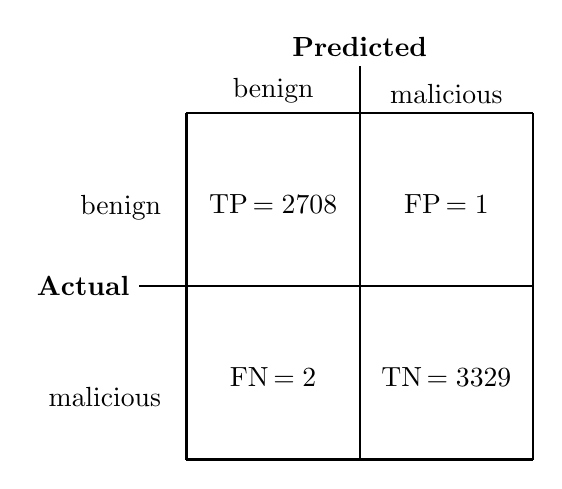
\begin{tikzpicture}[scale=2] %font=\scriptsize
		% Draw Basic Box
		\draw[thick] (0,0) -- (2.2,0);
		\draw[thick] (0,0) -- (0, 2.2);
		\draw[thick] (2.2,2.2) -- (2.2, 0);
		\draw[thick] (2.2,2.2) -- (0, 2.2);

		% Draw Box Ticks
		\draw[thick] (-0.3, 1.1) -- (2.2, 1.1);
		\draw[thick] (1.1, 0) -- (1.1, 2.5);

		% Box Labels
		% -- left side
		\coordinate[label=left:benign] (p1) at (-0.1,1.6);
		\coordinate[label=left:malicious] (p2) at (-0.1,0.4);

		% -- top side
		\coordinate[label=above:benign] (p3) at (0.55, 2.2);
		\coordinate[label=above:malicious] (p4) at (1.65, 2.2);

		% -- overall headers
		\coordinate[label=above:\textbf{Predicted}] (p5) at (1.1, 2.5);
		\coordinate[label=left:\textbf{Actual}] (p6) at (-0.3, 1.1);

		% Category Values
		\coordinate[label={TP$\,=2708$}] (TP) at (0.55, 1.50);
		\coordinate[label={FP$\,=1$}] (FP) at (1.65, 1.50);
		\coordinate[label={FN$\,=2$}] (FN) at (0.55, 0.40);
		\coordinate[label={TN$\,=3329$}] (TN) at (1.65, 0.40);
	\end{tikzpicture}
\end{center}

Additionally we generated a confusion matrix to observe the presence of FP and FN. The results of testing on 6640 samples (30\% of the dataset) show an accuracy of \textbf{99,95\%} for the trained model using \textit{Random Forest Classifier} with 100 estimators. Of course there are some minor corner cases, when the detection fails: 2 files were detected as benign while they are malicious and 1 benign file was predicted as malicious. However, the overall results (see Table \ref{table:results}) demonstrate that the obtained model can be efficiently applied for malicious PDF files detection.

\begin{table}[H]
	\caption{Random Forest Classifier performance results}
	\label{table:results}
        \centering
            \begin{tabular}{c c c}
                \toprule
                
				\textbf{Accuracy} & \textbf{Recall} & \textbf{F1-Score} \\
				\hline 
                0.995 & 0.9992 & 0.9994 \\
                
                \bottomrule
			\end{tabular}
\end{table}

% Classifier Performance Comparison + maybe add SVM (file:///C:/Users/viorel/Desktop/Bachelor/Resources/Malicious_PDF_Detection_ACSAC_12.pdf)

\newpage

\section{Used technologies}
\label{section:technologies}
\subsection{Microsoft .NET Framework}
As previously mentioned in sections \ref{section:backgroundProc} and \ref{section:filesystem}, our application is going to have a help tool for Windows based computers that will automatically detect new downloaded PDF documents, upload them to our Cloud Analyzer and take action (keep/delete) on that files corresponding to their category (benign/malicious). This tool will take the form of a Windows Service which will start running at the boot-time of the computer in the Session 0 (see section \ref{section:backgroundProc}) and will communicate with an application responsible for notifying users through Windows notifications (see Figure \ref{winserviceDesign}). 

\begin{figure}[H]
	\centerline{\includegraphics[scale=0.6]{figures/winService.png}}  
	\caption{Architecture's outline of the help tool for Windows}
	\label{winserviceDesign}
\end{figure}

Microsoft \textbf{.NET Framework} provides all the necessary Classes for creating the described tool. This framework represents a solution for standardization of application development on Windows operating system. Prior to the introduction of .NET Framework, the developers mostly used COMs\footnote{Component Objcet Model (COM) is a model of reusable software introduced by Microsoft in 1993} as a solution for code reuse. However, COM requires developers to write boilerplate code in order to turn their business logic into a reusable component, including memory clean up, reference counting etc, whence result a lot of errors. .NET Framework allow developers to focus on writing the business logic, while it is dealing with the memory management and is providing consistent exception-handling mechanisms. For example, in our application we implemented several .NET interfaces to achieve the expected behavior without having to manage a lot of low-level details. To create a Windows Service, we derived our class from \code{System.ServiceProcess.ServiceBase} and we had to override it's \code{OnStart}, \code{OnStop} methods. Because a service runs in Session 0, it means that it does not have support for user interface. Yet the application is intended to push Windows notifications and to ensure this functionality we had to treat our tool as a client-server application. The Windows service establishes an interprocess communication with the client \textit{Tray Notification App} when a user logs in. For this mechanism the WCF\footnote{Windows Communication Foundation (WCF) is a set an API in the .NET Framework for building connected, service-oriented applications} framework is integrated, which allows sending data as asynchronous messages from one endpoint to another. WCF was chosen as communication layer because it provides the \textit{duplex} message exchanging pattern, where two processes establish a secure TCP connection and can send data in both directions. To make this working, it is necessary to just define used entities for communication as \textit{Data Contracts}, that will later serialize the metadata by the WCF serialization engine. Another important component that lies at the core of the WCF service is the monitor class that inherits from .NET \code{System.IO.FileSystemWatcher}. It's behavior was described in section \ref{section:filesystem} and basically we use it to monitor user's specified folders and to send events to the users via the WCF communication. At the top level, in order to catch sent events from the Windows Service, a hidden WPF\footnote{Windows Presentation Foundation (WPF) is a UI framework for desktop applications from .NET Framework} application starts communication with the service at the user's login. When a PDF document is downloaded into monitored folder the Windows Service throws an event that is displayed to the user in form of a Windows System Tray Notification.


\subsection{Scikit-learn Machine Learning Library}
It would be extremely inefficient to always reimplement each Machine Learning algorithm that is required for solving a specific problem. \textbf{Scikit-learn} is one of the well known and largely used ML libraries, that came across as a solution for code reusability and performance optimization. This open-source library was created above the already prepared "ecosystem" for Data Science - \textit{Python}. Even Python is just a programming language, there are a plenty of created libraries using Python, that are used on a daily basis by scientists. In terms of efficiency there are no doubts, that Scikit-learn would give way to other ML libraries. And all this beacause of it's underlying technologies. At the core it integrates:

\begin{itemize}
	\item \textit{Cython} - a compiled language that can bind compiled libraries, reaching high performance of the CPU;
	\item \textit{Numpy} - optimized Python module for working with large multidimensional arrays;
	\item \textit{Scipy} - a large collection of efficient algorithms for linear algebra, interpolation etc.
\end{itemize}

Till now, the Scikit-learn developers have supplied the library with various supervised and unsupervised algorithms, such as: regression, clustering, classification algorithms, as well as: Random Forest, Support Vector Machine etc. It is a perfect solution for both academic and commercial projects, because of the simple API that it provides, thus the generic implementation of the ML algorithms can be adapted to personal purposes. Also, Scikit-learn integrates well with other Python libraries, that consistently simplify the data analyisis process. Some of these libraries are: 

\begin{itemize}
	\item \textit{Pandas} - offers optimized data structures (\textit{DataFrames}) for manipulation of large datasets. We could simpy apply \textit{Min-Max Normalization} (see \ref{subsection:featureSelection}) on entire loaded dataset from a raw CSV file.
	\item \textit{Matplotlib} - used for data visualization and plotting. Learning Curves of the classifier can be better analyzed from a visual representation.
\end{itemize}


\subsection{Python Flask}
As soon as the heart of our application came to life - the ML model for detecting malicious PDFs we needed a way to make it publicly accessible. \textbf{Flask} is a microframework for web applications that helped us to make it possible. Comparing to other web frameworks, Flask is focused more on simplicity and extensibility, making the development much more oriented on solving own business case. This lightweight framework has no in-built database abstraction layer or object-relational mapping and neither any form validation or authentication, instead it supports third-party libraries that provide all enumerated functionalities and even more. Flask core includes basic functionality required by all web applications and gives an abstraction for creating request-response mechanism based on \textit{Werkzeug} library, which provides a collection of utilities for WSGI\footnote{Web Server Gateway Interface (WSGI) is a specification that describes the communication pattern between a web server and web applications} applications. Other implementation details can be easily integrated based on personal preferences. For example we used a NoSQL database in our application, having the possibility to choose from a large variaty of available mechanisms for data storage. \par
The created web service respects the requirements of a RESTful architectural design, Flask framework providing a simple mechanism for specifying routing and HTTP methods. For demonstration purposes we have listed below a minimalistic example of a REST HTTP Method (processes a file sent over a POST request and returns a JSON result) showing the Flask simplicity. One of the major advantages of this framework is the compatibility supported by nowadays giants of Cloud Computing. Our created web framework that exposes methods for uploading and PDF files and analyzing them, as well as visualizing history of scanned files, can be later deployed to Cloud services such as: Google Cloud Platform, IBM Bluemix, Microsoft Azure etc. 

\newpage

\begin{python}
from flask import Flask, jsonify, request
app = Flask(__name__)

@app.route('/api/file-upload', methods=['POST'])
def upload_file():
	file = request.files['file']
	file_status = file_controller.upload(file)
	response = jsonify({'message': file_status})
	response.status_code = 200
	return response

if __name__ == "__main__":
    app.run()
\end{python}


\subsection{ReactJS Framework}
In order to use the web service in a user friendly way, a modern graphical user interface (\textit{GUI}) is needed. The contemporary approach for developing a web GUI is to use a frontend JavaScript Framework. The range of choice is extremely large, e.g. \textit{Angular}, \textit{Vue.js}, \textit{Ember.js} etc., but finally we decided for \textbf{ReactJS}. Being deveveloped and mantained by Facebook, ReactJS has a fast growing community and is one of the trending JavaScript Frameworks for 2020. The need of using a framework for web GUI arises because of necessity for time-efficient development experience, standardized methods of programming, faster performance and robust memory management. As other frameworks, ReactJS is aimed to render data to the \textit{DOM}\footnote{Document Object Model (DOM) is the representation of a web page that can be manipulated using JavaScript} and to eliminate the subsequent page refreshes in a complex web application that constantly updates its data. This mechanism is provided by the concept of \textit{Virtual DOM} used in React, which involves constructing the representation of a web page in a virtual memory, where it uses the \textit{Reconciliation Algorithm}\footnote{is a diffing algorithm that compares the types of root elements and decides which element should be rerendered} to perform only the necessary updates before rendering the page into the browser. \par
The extensibility of React code is assured by \textit{Components}, that are rendered to specific elements in the DOM. These can be declared in two ways: functional and class-based, the main difference being in the "state" which can be hold only by a class-based component. The performance is influenced positively by the lifecycle methods in React Components. There are multiple lifecycle methods for controlling the state of a web page, but two of them that should be definetely took into consideration are \texttt{componentDidMount}, that is called once the data is fully loadded from a remote source, and \texttt{render} which is called every time the component's state gets updated. \par
Usually React requires the use of additional libraries for common functionalities like routing, state management and layout styling of the UI. For these purposes we used:

\begin{itemize}
	\item \textit{React Router} - is a routing library that keeps the user interface in sync with the corresponding URL. It manages the redirection, lazy code loading and dynamic route matching.
	\item \textit{Redux} - is a state management tool, that keeps tracking of each component's state and store them into a global place, so that data becomes more accessible from any component.
	\item \textit{Semantic-UI-React} - is a collection of UI standards defined as a singular style. Instead of recreating the layout of commonly used web elements (Buttons, Grids, Modals, Input Fields etc.), it is more efficient to use a library with all of those elements already created.
\end{itemize}


